%Copyright �  2019 Rice University, Christopher M Jermaine (cmj4@rice.edu), and Risa B Myers  (rbm2@rice.edu)
%
%Licensed under the Apache License, Version 2.0 (the "License");
%you may not use this file except in compliance with the License.
%You may obtain a copy of the License at
%
%    https://www.apache.org/licenses/LICENSE-2.0
%
%Unless required by applicable law or agreed to in writing, software
%distributed under the License is distributed on an "AS IS" BASIS,
%WITHOUT WARRANTIES OR CONDITIONS OF ANY KIND, either express or implied.
%See the License for the specific language governing permissions and
%limitations under the License.
\documentclass[11pt]{article}
%\documentclass[12pt]{amsart}
%\usepackage{latex8}
\usepackage{fullpage}
\usepackage{times}
\usepackage{url}
\usepackage[normalem]{ulem}
\usepackage{epsfig} 
%\usepackage{latexsym}
\usepackage{subfigure}
\usepackage{graphicx}
\usepackage{titlesec}
\usepackage{multirow}

\titlespacing{\section}{0pt}{3mm}{1mm}
\titlespacing{\subsection}{0pt}{2mm}{0.5mm}
\titlespacing{\subsubsection}{0pt}{2mm}{0.8mm}

%\topmargin 0.75in 
%\oddsidemargin -0.04in
%\textwidth 6.5in
%\textheight 9.0in 
%\setlength{\textheight}{23.1cm}
%\setlength{\textwidth}{17.0cm}

\newcommand{\muhat}{\hat{\mu}}
\newcommand{\sigmahat}{\hat{\sigma}}
\newcommand{\todo}[1]{[\textbf{TODO: #1}]}
\newcommand{\eat}[1]{} % TO MAKE LARGE BLOCKS OF TEXT INVISIBLE
\newcommand{\sz}[1]{\lvert#1\rvert}
\newcommand{\card}[1]{\lvert#1\rvert}
\newcommand{\xp}[2]{P \if*#1\else^{#1}\fi \if*#2\else_{\! #2}\fi}
\newcommand{\pr}[3]{\xp{#1}{#2}\left\{\,#3\,\right\}}
\newcommand{\prl}[3]{\xp{#1}{#2}\{\,#3\,\}}
\renewcommand\:{\colon} % for use with \sset, etc.
\newcommand{\sset}[1]{\left\{\,#1\,\right\}}
\newcommand\xD{\mathcal{D}}
\newcommand\xP{\mathcal{P}}
\newcommand\xS{\mathcal{S}}
\newcommand\xbar{\bar x}
\newcommand\vbar{\bar v}
\newcommand\xmax{{x_{\text{max}}}}
\newcommand\eps{\epsilon}
\newcommand{\eeblk}{\hbox{\lower 1pt \vbox{\hrule width6pt\hbox to
  6pt{\vrule height5pt depth1pt \hfil\vrule height5pt depth1pt} \hrule
  width6pt} \unskip}}
\newcommand{\eblk}{{\unskip\nobreak\hfil\penalty50
  \hskip1em\hbox{}\nobreak\hfil\eeblk
  \parfillskip=0pt\finalhyphendemerits=0\par}}
\newtheorem{xample}{Example}
%\newenvironment{example}{\begin{xample}\em}{\eblk\end{xample}}
\makeatletter
\newenvironment{sql}%
 {\vskip 5pt\begin{list}{}{%
  \setlength{\topsep}{0pt}\setlength{\partopsep}{0pt}\setlength{\parskip}{0pt}%
  \setlength{\parsep}{0pt}\setlength{\labelwidth}{0pt}%
  \setlength{\rightmargin}{0pt}\setlength{\leftmargin}{0pt}%
  \setlength{\labelsep}{0pt}%
  \obeylines\@vobeyspaces\normalfont\ttfamily%
  \item[]}}
 {\end{list}\vskip5pt\noindent}
\makeatother
\newcommand{\bpar}[1]{\vskip 5pt\noindent\textbf{#1}\hskip 1em}
\newcommand\yN{{\tilde N}}
\newcommand\yX{{\tilde X}}
\newcommand\ymu{{\tilde\mu}}
\newcommand\ysigma{{\tilde\sigma}}


\newcommand{\goodgap}{
        \hspace{\subfigtopskip}
        \hspace{\subfigbottomskip}
}

%\renewcommand{\baselinestretch}{0.99}

\newtheorem{definition}{Definition}
\newtheorem{Rule}{Rule}
\newtheorem{lemma}{Lemma}
\newtheorem{theorem}{Theorem}
\newtheorem{problem}{Problem}
\newtheorem{example}{Example}
\newtheorem{optimization}{Optimization}
\newtheorem{observation}{Observation}
\newtheorem{corollary}{Corollary}

\newcommand{\qed}{\hspace*{\fill}
           \vbox{\hrule\hbox{\vrule\squarebox{.667em}\vrule}\hrule}\smallskip}

\long\def \ignoreme#1{}

\def\qed{\hfill \mbox{\rule[0pt]{1.5ex}{1.5ex}}}



\begin{document}
%\maketitle
%\pagestyle{empty}

\begin{center}
{\bf \huge{Introduction to Spark}}
\end{center}


\vspace{10 pt}

\section{Description}

The goal of this part of the assignment is to learn to do some distributed computing using Spark and PySpark.  

There are 2 different datasets that you will use:
\begin{enumerate}
\item Rx dataset: Medication prescriptions in the United Kingdom from  July 2016 to September 2017
\item Bioinformatics dataset: Tardigrade and bacteria genome sequences
\end{enumerate}

There are 3 tasks:
\begin{itemize}
\item Rx dataset
\begin{enumerate}
\item[1]  Compute the total ``net ingredient cost" of prescription items dispensed for each PERIOD 
\item[2] Compute the 5 practices that issued the prescriptions with the highest total net ingredient cost
\end{enumerate}
\item Bioinformatics dataset
\begin{enumerate}
\item[3]  Compute and label each sequence from a provided sample as most likely being Tardigrade or bacterial using Edit Distance.
\end{enumerate}
\end{itemize}
\section{Datasets}
\subsection{Rx Dataset}

The data set itself is a set of simple text files.  Each prescription/prescribing practice is a different line in a file. 
The attributes present on each line of the files are, in order:

\begin{center}
\begin{tabular}{ |l|l| } 
\hline
Attribute & Description \\
\hline
\texttt{SHA} &	Area team identifier  \\
\texttt{PCT}	 & Clinical commissioning group identifier  \\
\texttt{PRACTICE}	 & Practice identifier  \\
\texttt{BNF\_CODE}	 &British National Formulary (BNF) code  \\
\texttt{BNF\_NAME}	 & BNF name  \\
\texttt{ITEMS}	 & Number of prescription items dispensed  \\
\texttt{NIC}	 & Net ingredient cost (pounds and pence)  \\
\texttt{ACT\_COST}	 &Actual cost (pounds and pence)  \\
\texttt{QUANTITY}	 & Quantity - whole numbers \\
\texttt{PERIOD}	 &YYYYMM  \\
\hline
\end{tabular}
\end{center}

The data files are in comma separated values (CSV) format.
 It is stored as fifteen different files.

\noindent This is about 21 GB of data in all.  Important note: be aware that the URLs may not copy-and-paste from
this PDF correctly, as you may
lose underscore characters.  This problem may happen with the other commands below.


\noindent For testing and development, you can run your Spark jobs on just one of the fifteen files. 

A super-small subset of the first file (only about 1000 lines) is available for download (see Canvas).  This file may be used on your computer using Docker and the Spark container. If you want, you can also use this file for testing and debugging by loading it into HDFS (just like you did in lab) and then running your Spark program over it. 


\subsection{DNA Sequence Dataset}

\subsubsection*{Background}
Genomes are sequenced to help us better understand the genetic make-up of an individual or organism. The basic process involves taking a DNA sample (e.g. saliva), breaking it up into small pieces, choosing random fragments, determining the genetic composition of the fragments, and then ordering the fragments into a coded sequence. The machines used to sequence genomes are expensive, and are often provided as a service to an organization or as a remote lab. The following diagram from the National Human Genome Research Institute illustrates the process. \\

\begin{centering}
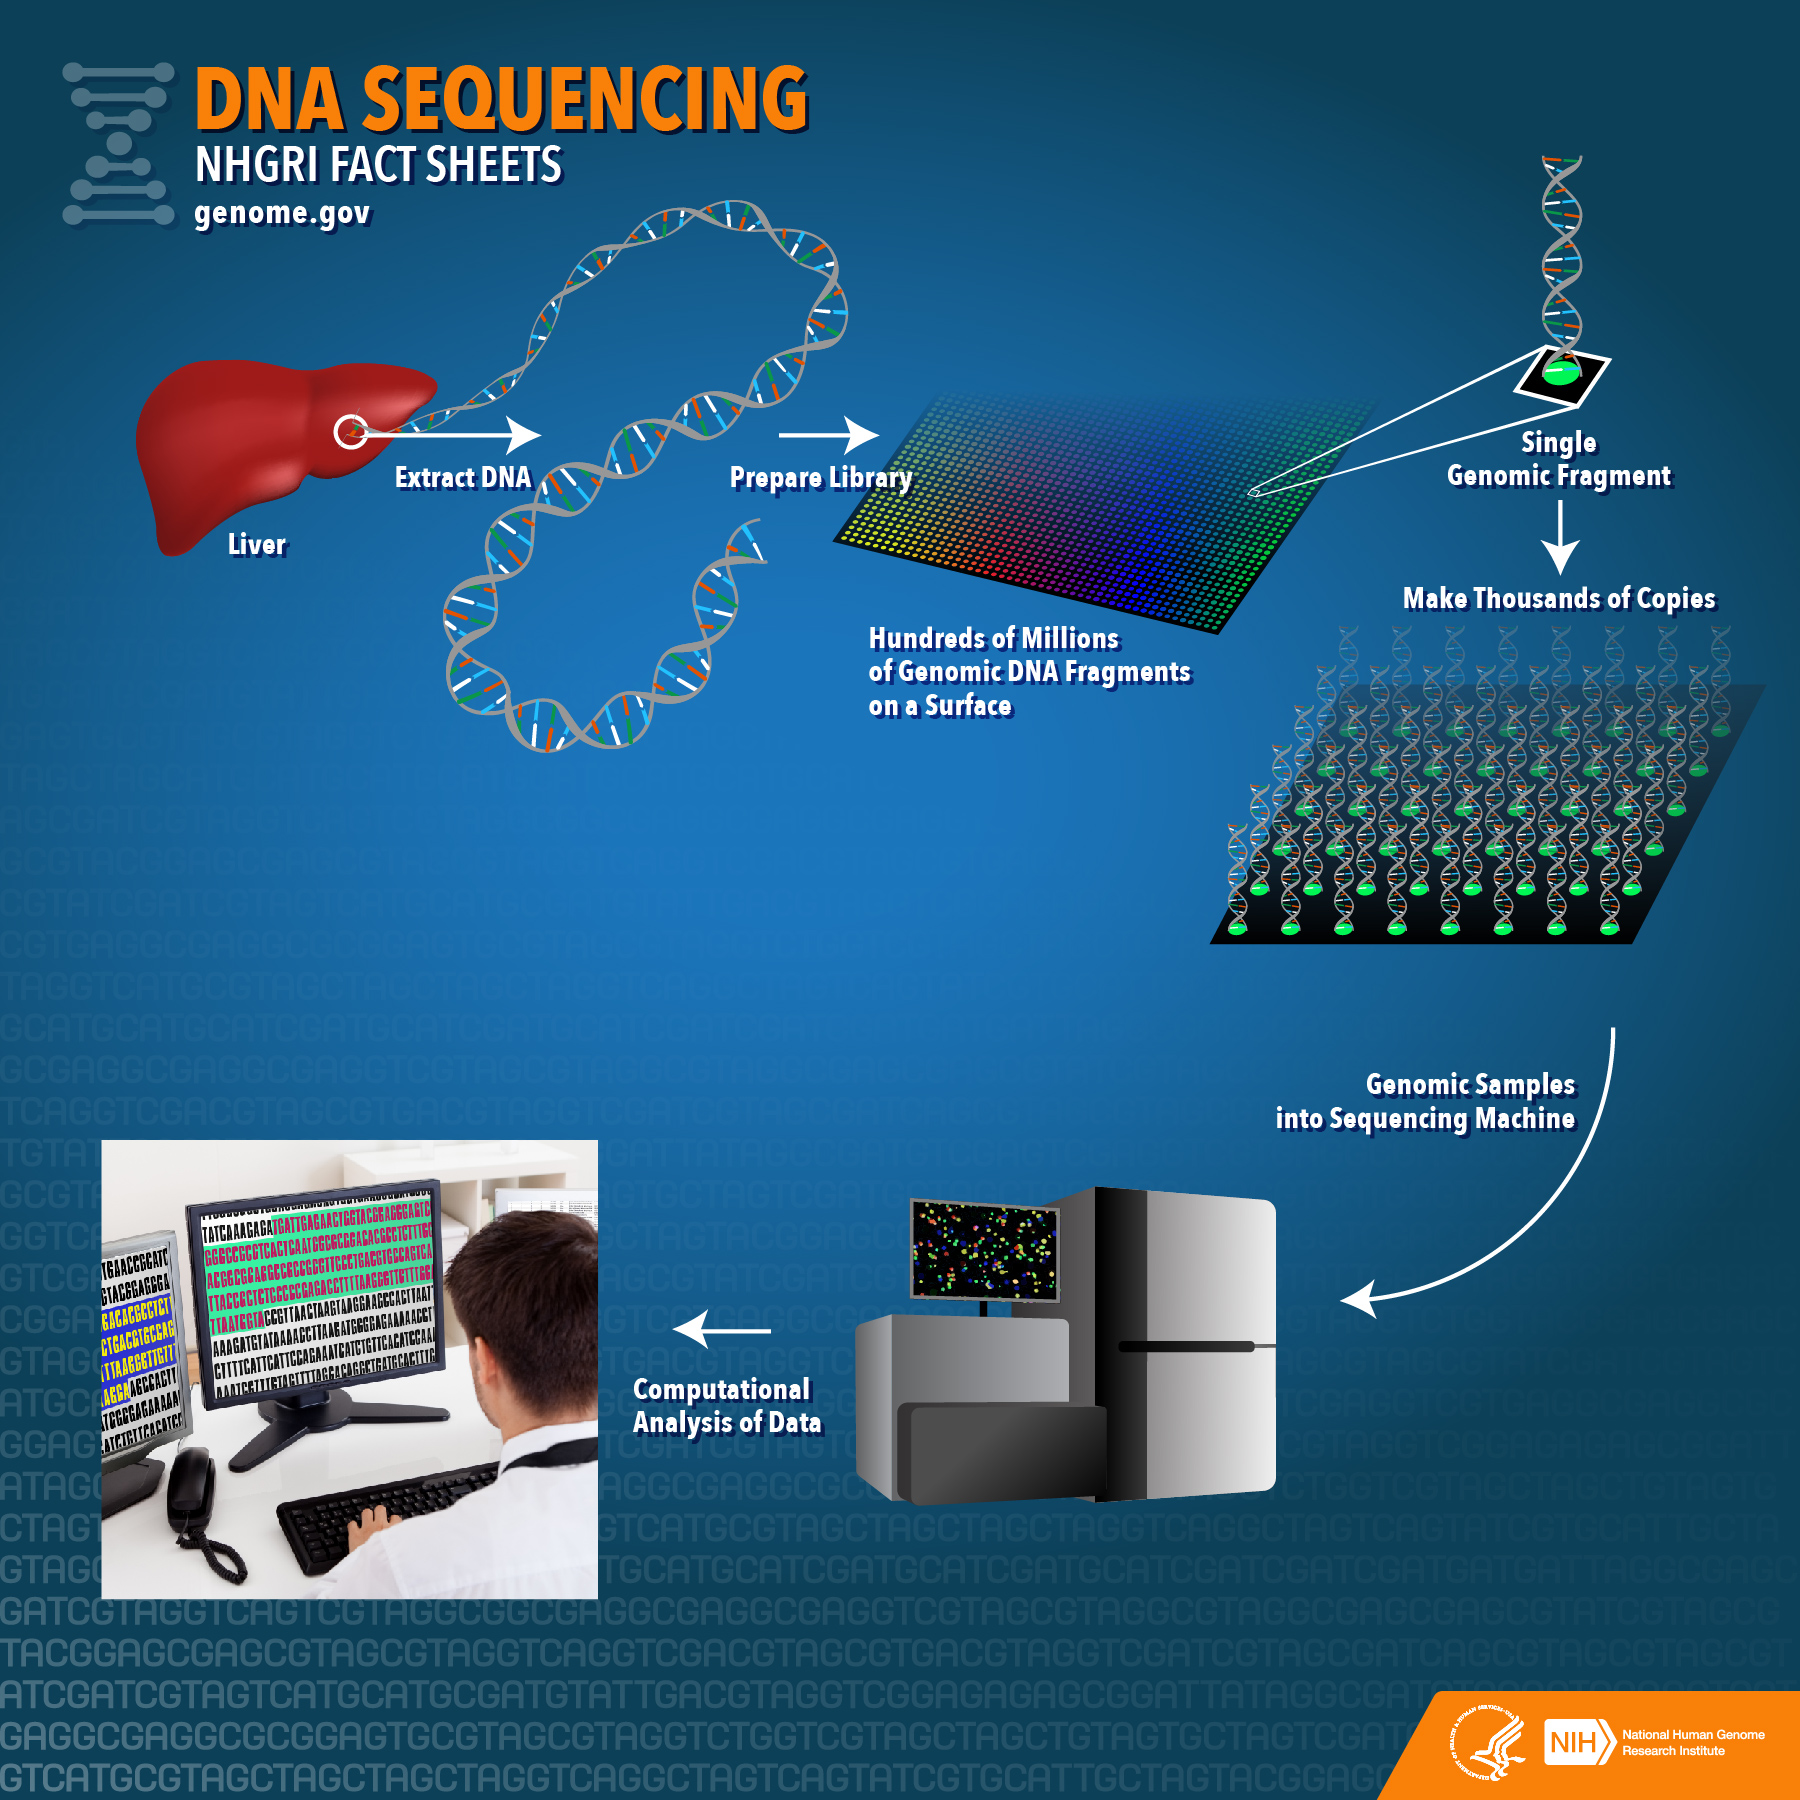
\includegraphics[width=0.6\textwidth]{dna_sequencing.jpg}
\end{centering}

%https://www.genome.gov/images/content/dna_sequencing.jpg

Consequently, there is the risk of contamination at many steps of the process when a genome is sequenced. When contaminated, genetic material from other organisms are introduced into the sample,  and are included in the assemblies that are output from the sequencing device.  Including this genetic content in the genome of the target organism can be misleading and lead to errors in research or diagnosis.

In this assignment, we will examine the assemblies from a contaminated tardigrade genome. We will compare the coded assemblies (or ``contigs'') with codes from a clean tardigrade set of assemblies as well as with codes from a number of bacteria.

The goal is to determine, for each coded segment of the contaminated sequence, whether or not it is likely to be bacteria or actual tardigrade DNA.

\subsubsection*{Tardigrades}
What is a tardigrade and why are we looking at this problem?

Tardigrades, also known as ``water bears'' are micro-animals that live in the water. They are caterpillar-like, with 4 pairs of legs and segmented bodies. They are ubiquitous and resilient. They have found just about everywhere in the world.  (\url{https://en.wikipedia.org/wiki/Tardigrade})

In 2015, Boothby et al. published a paper claiming that the tardigrade's ability to survive extreme conditions is due to horizontal gene transfer (HGT)(transfer of genetic material between species) from many different species, including bacteria, fungi, and plants \cite{boothby}. 

Koutsovoulos et al. investigated Boothby's claim and rebutted it. Basically claiming that the evidence seen was DNA sample contamination, not actual HGT\cite{Koutsovoulos}.

All of these papers (including the appendix for the rebuttal) are included in the assignment.

\subsubsection*{The data}
\begin{itemize}
\item The contaminated tardigrade assemblies are in \\
 \texttt{s3://risamyersbucket/tardigrade/LMYF01.1.oneline.fa}. \\
You will be comparing these contigs with contigs in the following other files:

\item The ``clean'' tardigrade reference assemblies are in the file \\
 \texttt{s3://risamyersbucket/tardigrade/nHd.2.3.abv500.oneline.fa}. 
\item Bacterial contigs are in the file \\
\texttt{s3://risamyersbucket/tardigrade/exp1.oneline.fa}. 
\end{itemize}

Each file contains a set of lines, one line per contig. Valid lines start with the `$>$' symbol, followed by the organism name. Next is a vertical bar (`$|$') followed by a unique identifier for the contig within the organism. There may then be additional text describing the contig. Finally, there will be a `$<$' symbol. After this symbol, the remaining text on the line contains the DNA code. As you may know, this text consists of the characters A, C, T, and G.

Valid contig lines start with a `$>$' and contain only the specified letters in the DNA code.
You should only include valid lines in your analysis.


\section{The Tasks}

There are three programming tasks associated with this part of the assignment. They involve analysis on the datasets.

\subsection{Task 1: 35 Points}

Write a PySpark program that checks all of the files and computes the total ``net ingredient cost" of prescription items dispensed for each PERIOD in the data set (total pounds and pence from the NIC field). 

As you do this, be aware that this data (like all real data) can be quite noisy and dirty.  The first line in the file might
describe the schema, and so it doesn't have any valid data, just a bunch of text. 
You may  find lines that do not have enough entries on them, or where an entry is of the wrong type (for example,
the NIC or ACT\_COST cannot be converted into a  decimal number.  Basically, you need to write robust code.
If you find any error on a line, simply discard the line.
Your code should still output the correct result.

For your results, print out each period, in sorted order, followed by the total net ingredient cost for that period.



\subsection{Task 2: 30 Points}

Write a PySpark program that computes the 5 practices that issued the prescriptions with the highest total net ingredient cost in the data set.
 This is actually quite simple to do, and very similar to Task 1.

\subsection{Task 3: 35 Points}

Your task is to classify each sequence in the contaminated tardigrade file as being most likely bacteria or tardigrade.  To measure the similarity of two sequences, you will compute the Edit Distance (https://en.wikipedia.org/wiki/Edit\_distance). Concretely, you need to write a function calculating the minimum amount of steps that is required to transform a sequence into the other, given two sequences. Some examples:
\begin{table}[h]
\centering
\begin{tabular}{|l|l|l|l|}
\hline
Sequence A    & ACCTTGC & CTGCCAA & ACTGCTG \\ \hline
Sequence B    & \underline{C}CCTT\underline{A}C & CTGCCAA & \underline{CTGCTGA} \\ \hline
Edit Distance & 2       & 0       & 7       \\ \hline
\end{tabular}
\end{table}

Note that since sequences in the data are all truncated to a same length. Your function does not have to be too complicated.

Then, for each sample sequence:
\begin{itemize}
\item Compute the Edit Distance against all the clean and bacterial sequences
\item Find the group of sequences that have the shortest distance
\item Label the sample as the majority of the group, or ``Not sure" in case of a tie
\end{itemize}

Some examples:

\begin{table}[h]
\centering
\begin{tabular}{cc|c|c|c|c|}
\cline{3-6}
                                                &       & \multicolumn{4}{c|}{Contaminated Sample}          \\ \cline{3-6} 
                                                &       & ACTGA      & ACCTT      & GCCAA      & GTGCA      \\ \hline
\multicolumn{1}{|c|}{\multirow{2}{*}{Clean}}    & CCAGG & \textbf{3} & 4          & 4          & 5          \\ \cline{2-6} 
\multicolumn{1}{|c|}{}                          & GCAAA & \textbf{3} & 4          & \textbf{1} & \textbf{3} \\ \hline
\multicolumn{1}{|c|}{\multirow{2}{*}{Bacteria}} & ACGCT & \textbf{3} & \textbf{2} & 4          & \textbf{3} \\ \cline{2-6} 
\multicolumn{1}{|c|}{}                          & TATCG & 4          & 5          & 5          & 4          \\ \hline
\multicolumn{2}{|c|}{Label}                             & Clean      & Bacterial  & Clean      & Not Sure   \\ \hline
\end{tabular}
\end{table}

Once you labeled the contaminated sample set, answer the following question:
\begin{enumerate}
\item If you are working on subset dataset, please print all the classifications. For full dataset, please give the classification[Clean, Bacterial, or Not Sure] for the following contigs instead:
\begin{enumerate}
\item LMYF01000203.1
\item LMYF01002593.1
\item LMYF01004256.1
\item LMYF01007394.1
\item LMYF01009100.1
\end{enumerate}

\item How many sequences in the contaminated file are believed to be bacterial sequences?

\end{enumerate}



\section{Important Considerations}

\subsection{Small data vs. big data}
We have provided a small subset of the data that you can use locally to develop and test your code.
However, to get full credit, you must run your code on the full datasets.

\subsection{Machines to Use}

One thing to be aware of is that you can choose virtually any configuration for your EMR cluster---you can choose different numbers
of machines, and different configurations of those machines.  And each is going to cost you differently!  Pricing information
is available at:

\vspace{10 pt}
{\footnotesize\texttt{http://aws.amazon.com/elasticmapreduce/pricing/}}  

\vspace{10 pt}
Since this is real money, it makes sense to 
develop your code and run your jobs on a small fraction of the data.
Once things are working, you'll then use the entire data set.
We are going to ask you to run your Spark code over the ``real'' data using two c3.2xlarge machines as
workers.

This provides 8 cores per machine (16 cores total) so it is quite a bit of horsepower. 

Be very careful, and shut down
your cluster as soon as you are done working.  You can always create a new one easily when you begin your work again.

\section*{Academic Honesty}
The following level of collaboration is allowed on this assignment: 

You may discuss the assignment with your classmates at a high level. Any issues getting Spark running is totally fine. What is not allowed is direct examination of anyone else's code (on a computer, email, whiteboard, etc.) or allowing anyone else to see your code. You may also use (and in fact are encouraged to use) the Spark reference manual \begin{verbatim}https://spark.apache.org/docs/2.3.1/\end{verbatim}

You may use the search engine of your choice to look up the syntax for Spark commands, but may not use it to find answers.

You MAY post and discuss results with your classmates. 

\section{Turnin}

Create a single document that has results for all three tasks and a screenshot indicating that you used 16 cores on AWS.
Then zip up all of your code and the document (use .gz or .zip only, please!), or else attach each piece of code
as well as your document to your submission individually.  

\section{Grading}

If you get the right answer and your code is correct,
\textbf{and you make use of the 16 cores available in your cluster} to get parallelism using the Spark framework,
you get all of the points.  
If you don't get the right answer or your code is not correct or you don't make use of the cores,
you won't get all of the points; partial credit may be given
at the discretion of the grader.

\section*{Bibliography}
\bibliographystyle{elsarticle-num}			
\bibliography{tardigrade}

\end{document}
